\documentclass[a4]{scrartcl}
\usepackage[margin=3cm]{geometry}
\usepackage[francais]{babel}
\usepackage[utf8]{inputenc}
\usepackage{amsmath}
\usepackage{graphicx}
\usepackage{subcaption}
\usepackage[colorinlistoftodos]{todonotes}
\usepackage{tabularx}
\usepackage{colortbl}
\usepackage{hyperref}


% define title
\title{Réalité Virtuelle}
\subtitle{Étude documentaire}

\author{Corentin Smith}
\date{\today}

\begin{document}
\maketitle

\newpage
\tableofcontents

\newpage
\section{Introduction}

\section{Définition / Histoire}

\subsection{Naissance}

Le premier système pouvant s'apparenter à de la réalité virtuelle dans l'acception moderne du terme est sans doute le Sensorama de Morton Heilig \cite{Sensorama}. Il s'agit d'une station composée d'un écran

\begin{figure}[!h]
	\centering
	\begin{subfigure}{.4\textwidth}
	  \centering
	  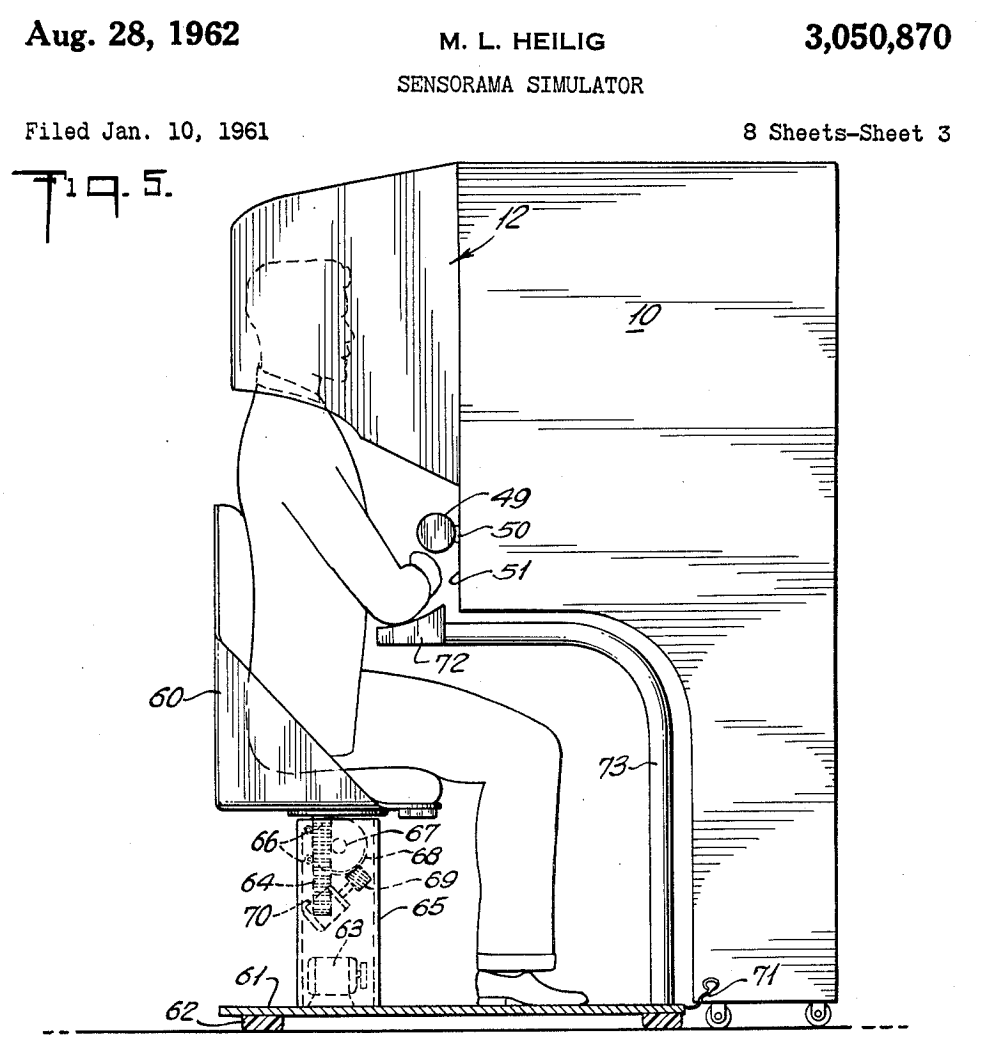
\includegraphics[width=\linewidth]{sensorama-patent}
	\end{subfigure}
	~
	\begin{subfigure}{.4\textwidth}
	  \centering
	  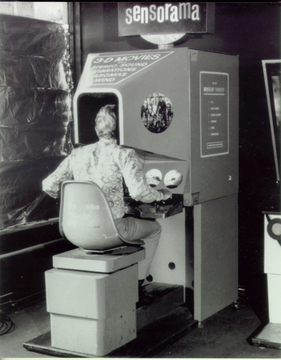
\includegraphics[width=0.8\linewidth]{sensorama}
	\end{subfigure}

 	\caption{Sensorama, Morton Heilig}
\end{figure}

\begin{figure}[!h]
	\centering
	\begin{subfigure}{.4\textwidth}
	  \centering
	  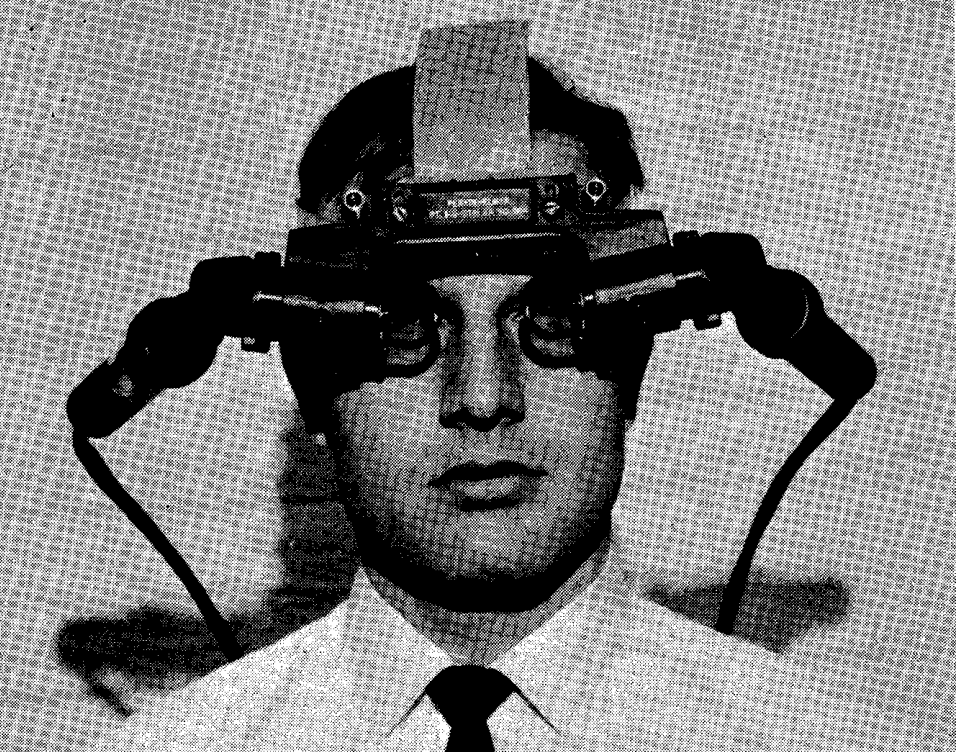
\includegraphics[width=\linewidth]{sutherland-1}
	\end{subfigure}
	~
	\begin{subfigure}{.4\textwidth}
	  \centering
	  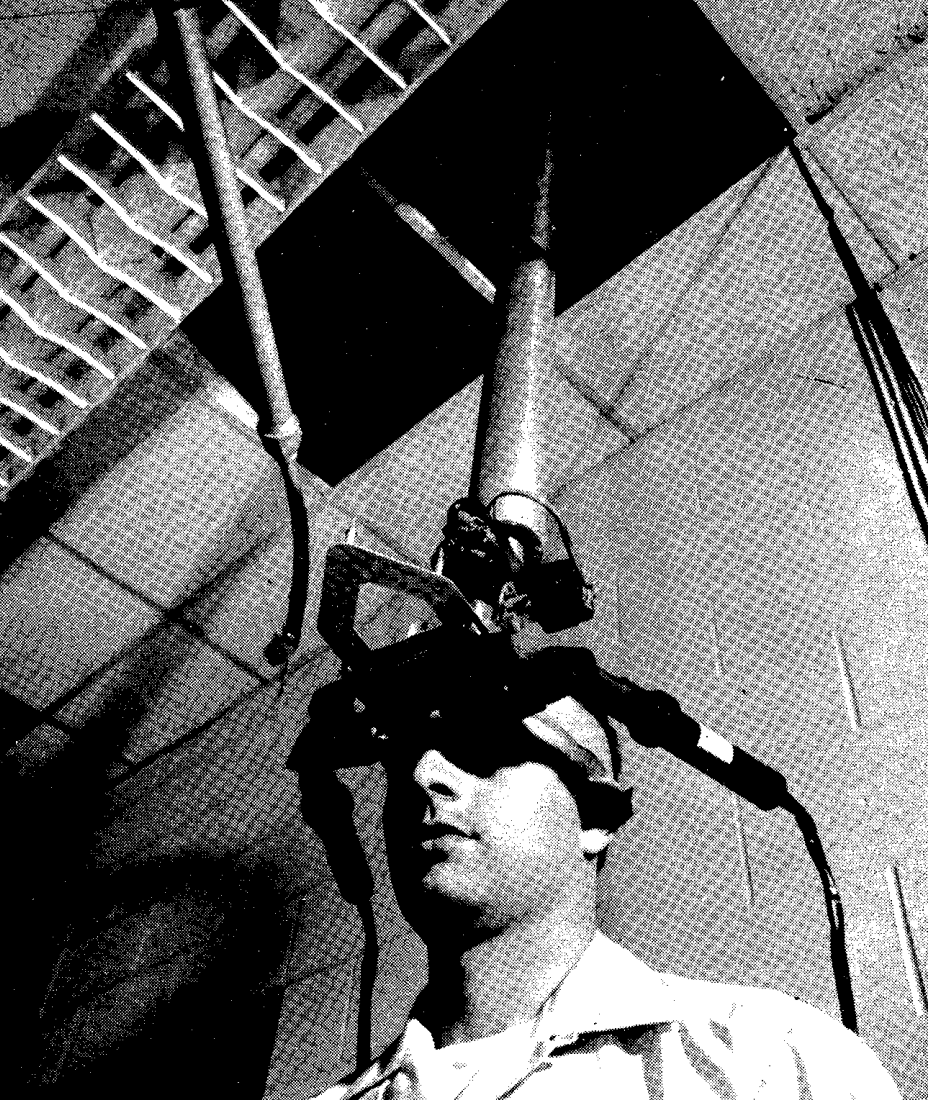
\includegraphics[width=0.8\linewidth]{sutherland-2}
	\end{subfigure}
 	\caption{Sutherland \cite{Sutherland68}}
\end{figure}

\begin{figure}[!h]
	\centering
	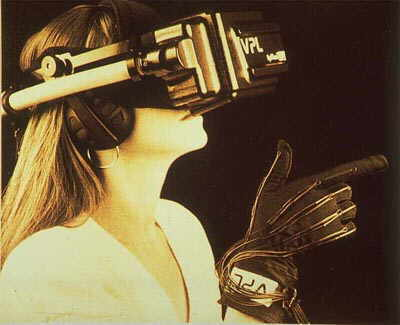
\includegraphics[width=0.6\linewidth]{vpl-hmd}
	\caption{VPL Research}
\end{figure}

Dans les années 80, la recherche s'intensifie, poussée notamment par des investissement de la NASA et du département américain de la défense [citation needed]

\subsection{Années 90}

\begin{figure}[!h]
	\centering
	\begin{subfigure}{.4\textwidth}
	  \centering
	  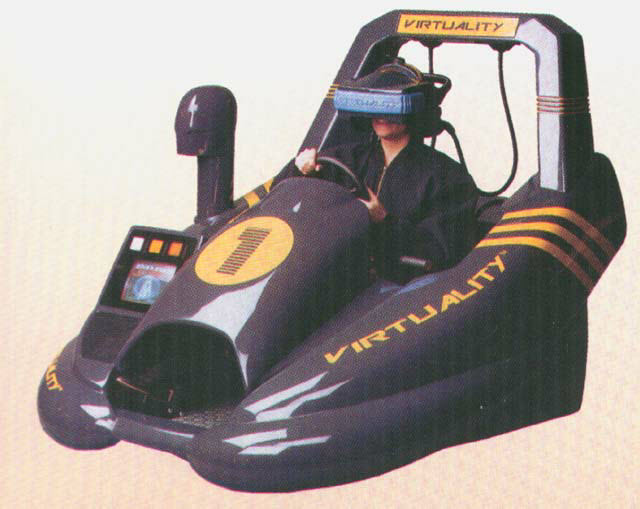
\includegraphics[width=\linewidth]{virtuality}
	  \caption{\emph{VR Pod} de Virtuality (1991)}
	\end{subfigure}
	~
	\begin{subfigure}{.4\textwidth}
	  \centering
	  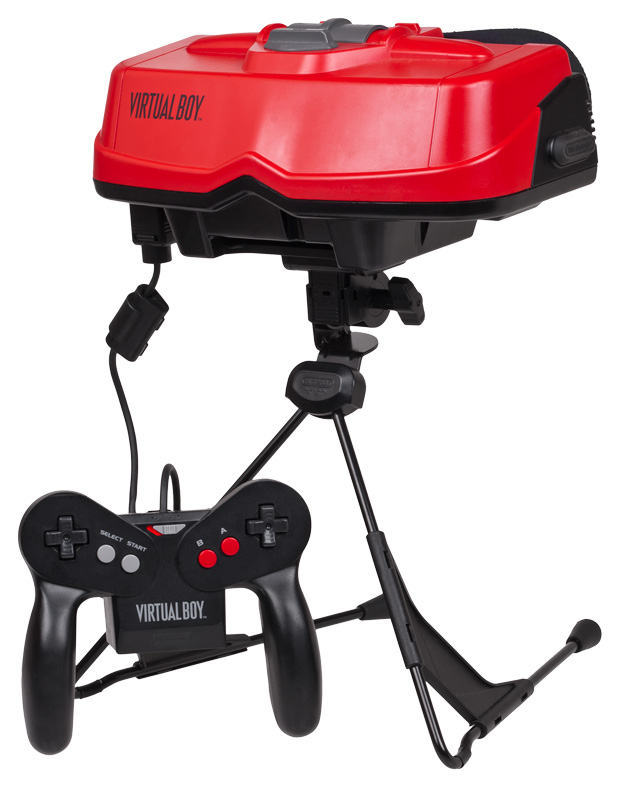
\includegraphics[width=0.8\linewidth]{virtualboy}
	  \caption{Nintendo Virtual Boy (1995)}
	\end{subfigure}
 	\caption{Systèmes de réalité virtuelle des années 90}
\end{figure}


En 1991, \emph{Virtuality} lance le premier système de réalité virtuelle grand public. Il comportait des lunettes et des gants à exosquelette, ce qui en fait la première expérience immersive de réalité virtuelle. Vendu pour environ \$60 000 l'unité, il est destiné principalement au salles d'arcades.

\subsection{Notion de présence}


\section{Technologie}


\subsection{Systèmes de vision}

Michael Abrash liste dans sa conférence \cite{Abrash14} les différents paramètres les plus importants à prendre en compte dans les systèmes de vision pour arriver à une sensation de présence.

\subsubsection{Champ de vision}

Le champ de vision est défini comme l'ouverture angulaire dans laquelle l'utilisateur peut voir la scène virtuelle. Selon Abrash, la présence commence aux environs de 80 degrés d'ouverture et s'améliore significativement vers 110 degrés. La plupart des appareils actuels ne dépassent pas 110 degrés de champ de vision.

\subsubsection{Résolution}

La résolution est un aspect évidemment très important d'une expérience de réalité virtuelle ; l'écran étant en général placé très proches des yeux de l'utilisateur, la résolution angulaire est assez faible en comparaison à un écran classique d'ordinateur ou de téléphone.

La résolution angulaire d'un \oe{}uil nu est de l'ordre d'une arcminute, ou $0,016$ degrés. Pour arriver à cette résolution angulaire avec un champ de vision de 110 degrés, il faudrait une résolution d'environ $6600 \times 6600$ (dans un format d'environ 4cm $\times$ 4cm si on place l'écran à une distance de 3cm de l'\oe{}uil, ce qui donne une densité de 4200 pixels par pouce).

On est donc encore loin d'être à ces niveaux de densité puisque les écrans les plus fins actuels arrivent tout juste à 500 pixels par pouce ; ce qui correspond au dernier prototype d'Oculus Rift, annoncé cette année au CES, qui est supposé avoir un écran de 2560 $\times$ 1440.

\subsubsection{Faible persistence}



\subsubsection{Haut taux de rafraichissement}


\subsubsection{Global display}


\subsubsection{Optique}


\subsubsection{Calibration optique}


\subsubsection{Tracking robuste}


\subsubsection{Temps de latence}

\cite{Abrash12} \cite{Carmack13} 


\subsection{Systèmes audio binauraux}


\subsection{Systèmes maîtres/esclaves}




\section{Développements récents et futurs}

\subsection{Oculus}
\subsection{Grand public enfin possible ?}


\newpage
\bibliography{bibliography}
\bibliographystyle{plain}


\end{document}





